\section{Evaluation and results}
\label{evares}

\subsection{Methodology used for experimentally evaluating the protocol}

To evaluate the new gossip protocols, they were tested in Cothority simulations and compared to the previous implementation under varying conditions.
These conditions include the number of nodes, the number of failing nodes, and an artificial message delay, which is used to simulate real-world network delays.
The delay for any given message was randomly picked from a uniform distribution between a fixed minimum and maximum delay.
A failing node, in our simulations, drops all incoming messages and sends no messages, effectively causing the node to be offline.
If a node is not failing, it is considered \emph{active} and functions correctly, the root was active in all simulations.
All experiments were run on a single machine with six 2.20~GHz Intel Core~i7 processors under Ubuntu~18.04.

Three metrics were used to evaluate the protocols.
The most important metric is the time it takes until the root returns the cosignature, called the \emph{protocol duration}.
The other two metrics we measured are the number of messages sent per active node and the amount of data sent per active node.
Both rumor messages and shutdown messages (when existing) are included in these metrics.


\subsection{Parameter values used in simulations}
\label{defaults}

The parameters come in two groups: environment parameters that are not within the node's control, and protocol parameters that affect how the nodes behave.

For the environment parameters, we simulated different combinations of total number of nodes and number of failing nodes, as explained in Table 1.

\begin{table}[]
  \caption{Number of nodes used in simulations}
\centering
\begin{tabular}{|c|c|}
\hline
Total number of nodes & Number of Failing nodes   \\ \hline
7                     & 0-2     \\ \hline
16                    & 0-5    \\ \hline
25                    & 0-8    \\ \hline
36                    & 0-11  \\ \hline
\end{tabular}
\end{table}

In addition to this, a small range of possible delays ($0.01$~seconds between the minimum and maximum delay) is specified to prevent unnatural effects where, for example, messages from different nodes always arrive at the same time.

\begin{itemize}
    \item Minimum message delay: $0.095$~seconds
    \item Maximum message delay: $0.105$~seconds
\end{itemize}

The threshold of signatories for a valid cosignature is always set to $n~-~\lfloor \frac{n-1}{3} \rfloor$ because this is the value that is used in ByzCoin.
The default values for the other protocol parameters are as follows.

\begin{itemize}
    \item Number of recipients for each rumor message: $r = 3$
    \item Interval between sending out rumor messages: $t = 0.07$~seconds
    \item Number of initial shutdown-message recipients: $s = 2$
\end{itemize}

These default values for protocol parameters were chosen as a compromise between protocol speed and efficiency.

The evaluation done has two parts, the first one is the comparison between the gossip protocol implementations, to see how the efficiency performance has improved or decreased. The second part compares the ONet Hybrid protocol with the existing gossip protocol, for evaluation of the difference that the implementation approach makes in the performance.

\subsection{Comparison of the gossip protocol implementations}

For the first part, the new gossip protocol was compared to BLS~CoSi with varying numbers of nodes and failing nodes, using the parameters mentioned in the previous paragraphs. The duration of the mask protocol was fairly stable, always measuring below 1.5~seconds in this set of experiments.
With very few failing nodes, it performs similar to the existing implementation, and with a high number of failing nodes, the mask protocol is only slightly slower (around 0.1 seconds).The mask aggregation protocol had a larger protocol duration in all the scenarios.
The timings are shown for $n = 36$ in Figure~\ref{fig1time}. Each box goes from the first quartile to the third quartile. The horizontal line is the median.

\begin{figure}[H]
    \centering
    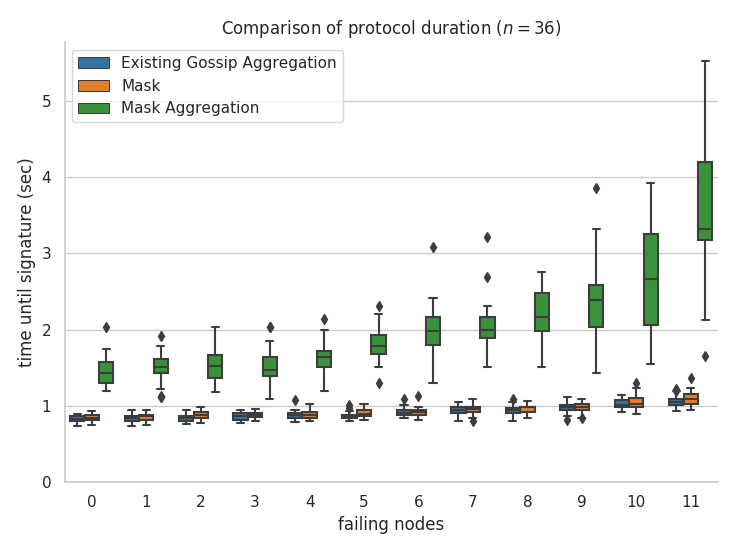
\includegraphics[width=1\textwidth]{images/aggregation_round_wall_sum_36.png}
    \caption{Timings until a cosignature was returned using the different variations of gossip protocol. }
    \label{fig1time}
\end{figure}

For $n = 36$, if we compare the number of messages sent by every node, as seen in Figure~\ref{fig1num}, both mask protocol and mask aggregation protocol send more messages than the existing implementation, since they send pull messages when possible, to get the signatures they need from other peers. Nevertheless, if we compare the amount of data transferred (bandwidth used) by every node, the mask protocol performs slightly better than the existing gossip aggregation, with a consistent improvement of 100kb per node, this can be observed in Figure~\ref{fig1data}. The mask aggregation protocol has a larger amount of bandwidth used, this might be caused by the constant pulling of all the different combination of multi-signatures that are available, so when a node has k signatures, there are $2^{k} - 1$ possible sets of combinations (excluding an empty set), and all of these are propagated by nodes requesting them when they know about them. This explains the increased bandwidth for the mask aggregation implementation.

\begin{figure}[H]
    \centering
    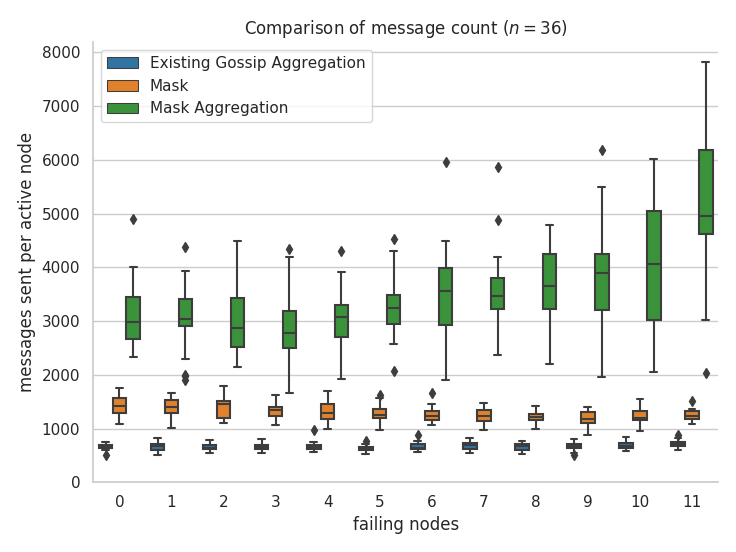
\includegraphics[width=0.91\textwidth]{images/aggregation_bandwidth_msg_tx_sum_36.png}
    \caption{Number of messages sent per active node using different variations of gossip protocol.}
    \label{fig1num}
\end{figure}

\begin{figure}[H]
    \centering
    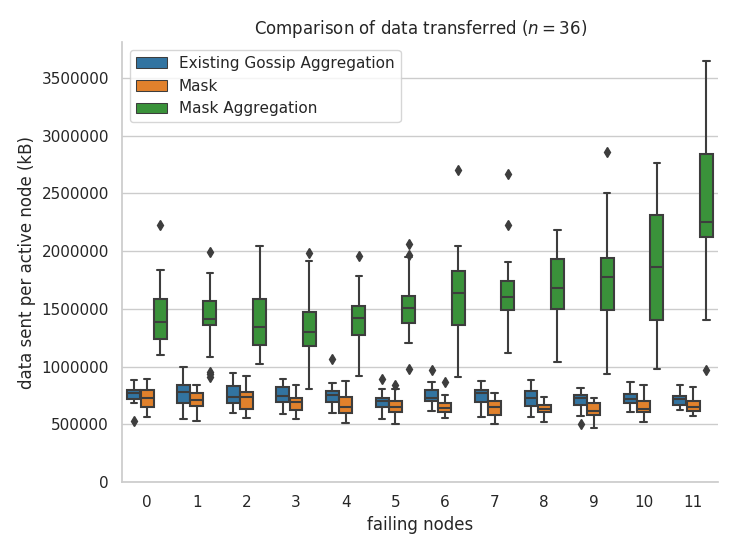
\includegraphics[width=0.91\textwidth]{images/aggregation_bandwidth_tx_sum_36.png}
    \caption{Amounts of data transferred per active node using different variations of gossip protocol.}
    \label{fig1data}
\end{figure}


Other results for simulations with different number of nodes, are available in the form of plots in Appendix~\ref{axresults}.

\subsection{Comparison of the ONet implementation with the existing gossip aggregation}

In the second part, the new ONet hybrid protocol is compared to the existing gossip protocol implementation with the same parameters mentioned earlier.
We can observe that the performance is improved in all the metrics, the number of messages and bandwidth used is decreased significantly, and the protocol duration also has a considerable improvement.
Here we can see the benefits of the Hybrid implementation, where we keep a low protocol duration (except for a single outlier that takes 0.2 seconds longer than the existing gossip implementation) and still have good efficiency in the quantity of messages and data sent when some nodes are failing.
These values are shown for $n = 36$ in Figure~\ref{fig2time}, Figure~\ref{fig2data}, and Figure~\ref{fig2num}.


\begin{figure}[H]
    \centering
    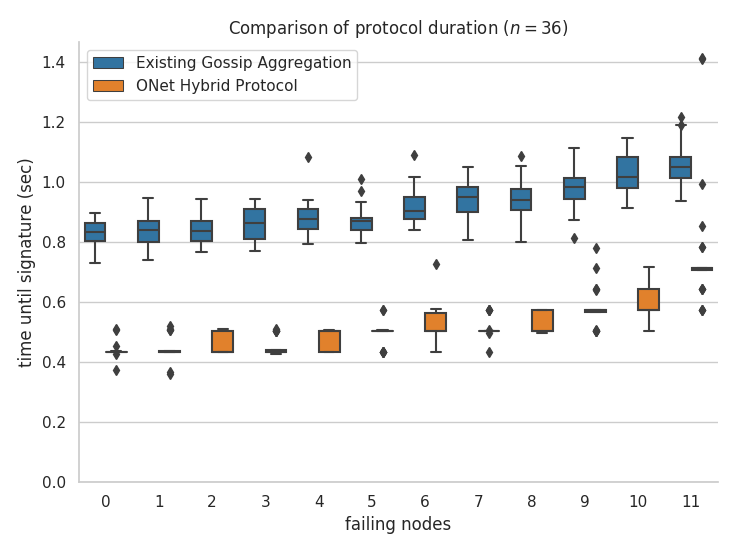
\includegraphics[width=0.91\textwidth]{images/round_wall_sum_36.png}
    \caption{Timings until a cosignature was returned using ONet Hybrid protocol vs Existing Gossip Aggregation.}
    \label{fig2time}
\end{figure}

\begin{figure}[H]
    \centering
    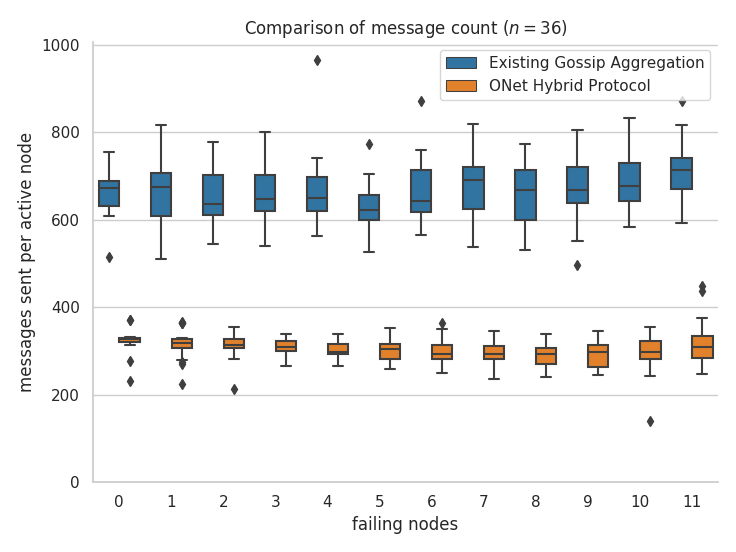
\includegraphics[width=0.91\textwidth]{images/bandwidth_msg_tx_sum_36.png}
    \caption{Number of messages sent per active node using ONet Hybrid protocol vs Existing Gossip Aggregation.}
    \label{fig2num}
\end{figure}

\begin{figure}[H]
    \centering
    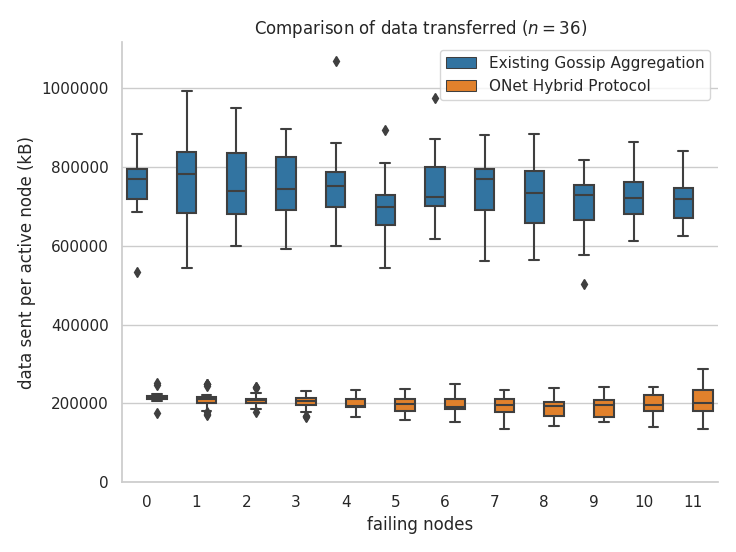
\includegraphics[width=0.91\textwidth]{images/bandwidth_tx_sum_36.png}
    \caption{Amounts of data transferred per active node using ONet Hybrid protocol vs Existing Gossip Aggregation.}
    \label{fig2data}
\end{figure}


